%``As we all know, the programmable computer, with its current speed and storage, is a gadget without precedent.
%It is a gadget that we may appreciate in many different ways:
%in this series of lectures I would like to appreciate it as the embodiment of an intellectual challenge that is also without precedent, viz.
%the challenge to program the gadgets.
%This challenge seems unique in the combination of the possibility for unmastered complexity
%-- programs are among the most complex things ever conceived --
%and the ultimate, but misleading, simplicity of a world of zeros and ones alone.''~\cite{dijkstra1979}
%These amazing advances in computer application can distract attention from the fact that Computer Science
%also has a central core of fundamental discoveries which are particular to itself as an independent
%intellectual discipline. Comput- ing Research is driven, like research in other mature branches of
%pure science, by natural curiosity, exploring the basic foundations and limitations of the pro- grammable computer,
%independent of any particular area of application. Because of its effective combination of pure knowledge
%and applied invention, Computer Science can reasonably be classified as a branch of Engineering Science.
%\cite{hoare2006}

There is a feature about programs that has always fascinated me immensely.
It is that there are \emph{multiple different ways} to write a program to compute the \emph{same result}.
Essentially, we fix the program input and output, but are free to change what happens in-between.
Software engineers will recognize this activity as the art of refactoring.
A more scientifically inclined reader will describe it as multiple algorithms compute the same function.

To demonstrate the idea, consider the two programs in~\autoref{lst:intro} where the variable \pr|bit| is either \(0\) or \(1\).
It is clear the programs look different.
Yet, I claim they compute equivalent results.

\begin{minipage}{\textwidth}
\begin{center}
\begin{minipage}{.3\textwidth}
\begin{lstlisting}[nolol,label={p1},frame=none,numbers=none,aboveskip=0pt,belowskip=0pt]
if (bit) { Z = X; }
else     { Z = Y; }
\end{lstlisting}
\end{minipage}\hspace{3em}%
\begin{minipage}{.4\textwidth}
\begin{lstlisting}[nolol,label={p2},frame=none,numbers=none,aboveskip=0pt,belowskip=0pt]
Z = X * bit + Y * (1 - bit);
\end{lstlisting}
\end{minipage}
\end{center}
\captionof{lstlisting}[Equivalent programs]{Equivalent programs.}
\label{lst:intro}
\end{minipage}

It is natural to ask \enquote{which one is better?}
The former is {easier} to understand {to a human};
a useful criteria if the program is intended for software engineers.
The latter has the benefit that it eliminates the conditional branching and evaluates in {constant time}, which is a desirable for program security.
Choosing the preferable program form therefore depends on the semantics -- what do we mean by \enquote{better}?
Moreover, how do we discover these alternative-but-equivalent ways to write a program?
We also need ways to confirm that the programs {actually} compute the same result, not just my claim!
 
Recognizing (and {embracing}) this ambiguity brings us to the world of program analysis and formal methods.
These are two foundational topics of this dissertation.
As the name implies, program analysis provides the techniques to inspect programs, and determine whether they satisfy some desirable criterion.
The general term for such criterion is a \emph{property}.
Formal methods complements the setting by adding the mathematical tools that we need to obtain rigorous guarantees.
With formal methods it is possible to provide \emph{proofs} for the analysis conclusions. 
Then, we can swap claims for confident assertions.

However, to make the exploration more adventurous and worthy of a multiyear doctoral study, we bring in \emph{implicit computational complexity} (ICC).
The topic is covered in detail in~\autoref{icc};
but briefly, ICC finds ways to characterize programs' runtime properties by introducing \emph{restrictions} at the level of programming languages.
This enables reasoning about program properties \emph{before} any program even exists.
Through the temporal shift, implicit complexity empowers us to think about properties as part of language \emph{design}, rather than an aposteriori activity.

Combining the three topics mentioned, we craft a setting where the goal is to \emph{analyze} programs, ideally with formal \emph{guarantees}, and starting with a \emph{programming language} that provides those guarantees \emph{by construction}.
Embedded in the setting is the assumption that when we restrict a language, we will not be able to write every program;
\ie we sacrifice Turing-completeness.
This naturally leads to the question, \enquote{what can we do with such a language?}\footnote{
See \url{https://stackoverflow.com/questions/315340} for an inspirational warm-up.}
Every manuscript of this dissertation is an instance responding to this broader question.

The existing works in implicit computational complexity focus primarily on \emph{defining} theoretical systems that ensure desirable runtime properties;
typically, in terms of computational resource usage (\cf~\autoref{tab:icc-results}).
What separates this dissertation from those works is that it never defines such systems;
rather, it centers on \emph{applications}.
In this view, we take the existing ICC systems as a baseline---a kind of metaphorical \enquote{toolbox}---and assess their utility.
Each dissertation manuscripts approaches this task by combining implicit computational complexity with some other application domain.
The task of expanding ICC outside its traditional (theoretical) realm is difficult for at least three reasons.

\begin{enumerate}

\item Taking any pure theory and applying it reveals the shortcomings of the theory, and those issues must then be resolved.

\item Broad insight is required to first identify suitable application domains and to convert theories to applications.
Evidence supporting this statement can be found, \eg in automata theory\footnote{
The classic formulation of Parikh's Theorem concerns language expressiveness.
However, its usefulness in applications was enabled {only decades later}, by the development of efficient algorithms.
Parikh's Theorem has since then been exploited in a range of applications, including SMT solvers, verification of cryptographic protocols and concurrent programs, and query evaluation over graph databases, to name a few~\cite[pg. 2]{hague2024}}.

\item Presenting the applications requires communicating the findings to (potentially new) audiences who are motivated differently to assess the {usefulness} of those findings.
\end{enumerate}

In other words, publishing findings involves a degree of technical evangelism: promoting implicit computational complexity to audiences who may have not encountered it previously (at least not in the presented way), and getting them excited about its \emph{application} potential.
After many decades of theoretical development, the quest for applications is critical to move implicit computational complexity forward~\cite[p.~7]{moyen2017}.
Through the effort, we gain insight of the technical power, limitations, and benefits of ICC systems as compared to alternative techniques; and like the manuscripts in this dissertation will demonstrate.

\subsection{Specific Aims}\label{subsec:specific-aims}

This dissertation has three scientific goals.

The first is to show that implicit computational complexity is useful in \emph{automated} complexity analysis.
All too often practitioners regard theory as irrelevant, and theoreticians think of practice as trivial;
but in reality, the two are symbiotic.
This goal shows the bidirectional importance of theory and practice that concurrently requires resolving various unexpected challenges. 
The findings are materialized in a series of manuscripts that extend the flow calculus of mwp-bounds (\autoref{flow-calculus}).

The second is to show that the analytical techniques developed around implicit computational complexity can be adjusted to track \emph{other} semantic properties.
This goal shows that ICC-based techniques are flexible enough to extend beyond their original design, and can accommodate numerous properties.
By extension, it suggests that the view of ICC as a niche subfield of complexity theory does not adequately recognize its true analytical power;
and that the extended applications should be explored more broadly.
The manuscripts in this dissertation show two cases of applications, in program optimization and security analysis.
 
The third goal is to strengthen the hypothesis that implicit computational complexity is naturally suited to formal reasoning.
Classic complexity theory is predicated on machine models that are difficult to represent formally~\footnote{
For example, a formal model of TMs in~\textcite{forster2020} took five years to complete.}.
In contrast, the programming languages-based approach of implicit computational complexity makes formal reasoning more accessible.
The findings of this dissertation are sufficient to motivate and justify the effort for undertaking rigorous formalization projects.

\begin{figure}[t]
\begin{mdframed}
\paragraph*{Main hypothesis.}
The utility of implicit computational complexity extends beyond \emph{theoretical reasoning} about the usage of computational resources.
\end{mdframed}
\caption[Main hypothesis summarized]
{Main hypothesis summarized.}
\label{fig:hypothesis}
\end{figure}

\subsection{Overview of the Dissertation Manuscripts}
\label{subsec:conn-papers}

The dissertation manuscripts stem from two works in implicit computational complexity.
Based on the origin, the manuscripts can be categorized in two disjoint tracks, as shown in~\autoref{fig:conn_papers}.
The tracks align with the three goals of~\autoref{subsec:specific-aims} as follows.

\begin{figure}[p]
    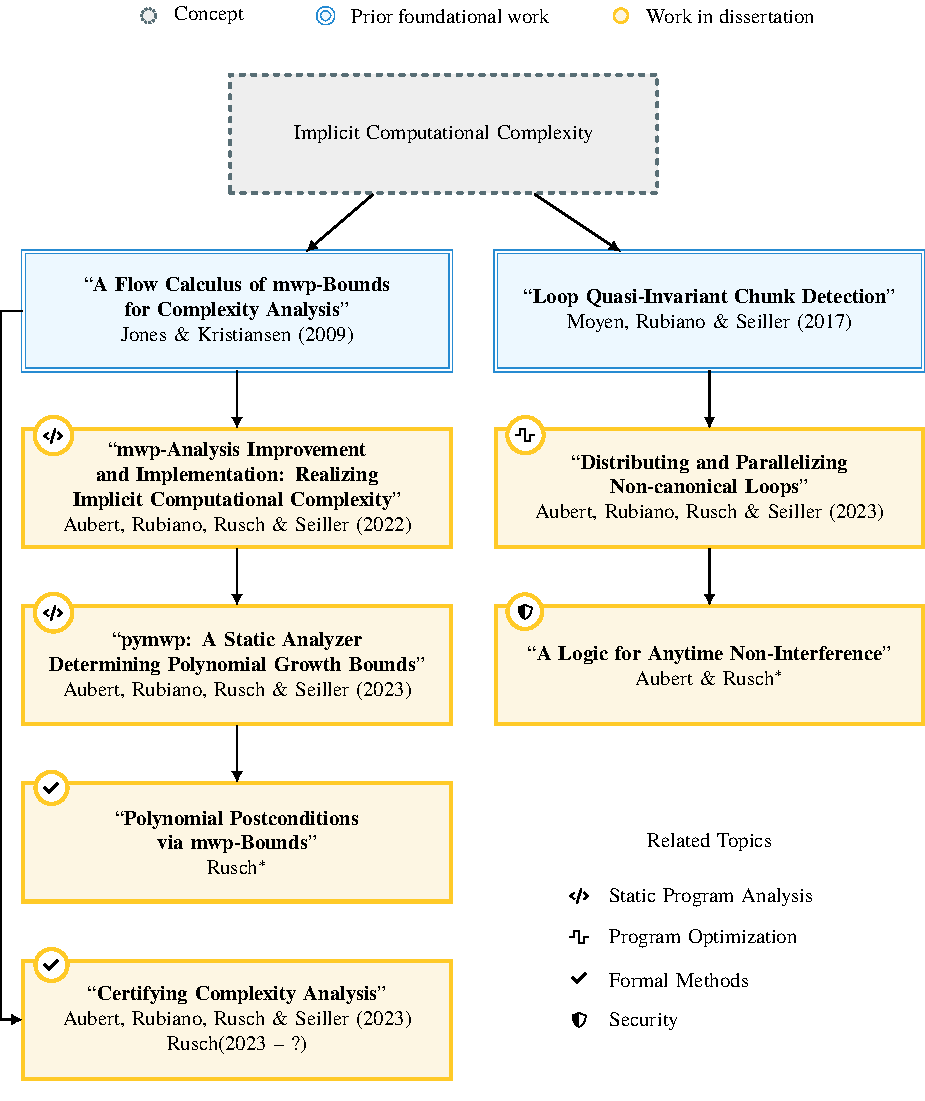
\includegraphics[width=\linewidth,keepaspectratio]{fig_conn_papers}
    \caption[Dissertation manuscripts]{Dissertation manuscripts.}
    \label{fig:conn_papers}
\end{figure}

\begin{description}
\item[Extensions of the flow calculus of mwp-bounds.]
The first track extends the flow calculus of mwp-bounds of~\textcite{jones2009}.
The technique is introduced detail in~\autoref{flow-calculus}.
The flow calculus is a syntactical analysis for reasoning about variable value growth during computation.
The manuscripts apply and demonstrate the utility of the calculus, first though static program analysis, then extending it to formal methods.
Thus, the manuscripts supports two of the three dissertation goals.
One of the manuscripts is in the appendix due to the university policies, but the placement should not distract from its significance;
several other manuscripts follow from it.

\item[Repurposing of Loop Quasi-Invariant Chunk Detection.]
The second track is inspired by \enquote{Loop Quasi-Invariant Chunk Detection}~\cite{moyen20172}.
The idea is to identify blocks of code in loops that become invariant after some finite number of loop iterations.
These quasi-invariant blocks can then be lifted from the loop to ideally improve the loop's complexity profile.
The manuscripts in this track support the second dissertation goal,
as they use the mathematical framework of LQICM to track other program properties.
In particular, they show how to adjust the mathematics to obtain a program optimization to increase parallelism and detect the security property of non-interference.
\end{description}

Each manuscript combines implicit computational complexity with some other topic in computer science.
The manuscripts are marked with thematic graphical icons that identify the related topic, among static program analysis, security, program optimization, and formal methods.
These icons will appear and are used with this designation throughout the dissertation.

% \subsection{Significance}\label{subsec:significance}

% This research proposal intersects computer science theory and application, with the intent of using those theoretical approaches to solve existing challenges in automatic program analysis.
% In 2017, Jean-Yves Moyen---a notable researcher in the ICC community, whose career spans 3 decades of advancements---remarked enthusiastically, that after twenty years and many results, ICC was ready to move into real-world and to concrete applications~\cite[p.~7]{moyen2017}.
% And although a few early results exist, as noted earlier in this section, progress in this direction is still at early stages.
% With similar aspirations, this proposal hopes to move further in that direction.
% It is conceivable that certified complexity would be of significant interest to multiple research communities.
% The next section will detail the specifics of the methodology, that consists of multiple projects.
% Assuming the successful completion of each project, they would show that certifiably correct complexity analysis is achievable, and that ICC techniques can be used to obtain efficient and practical complexity analysis.
% These results would extend current capabilities in automatic complexity analysis, and move those techniques closer to becoming a standard in real-world software verification.

\subsection{Tips for Interacting With This Document}
\label{subsec:tips}

\subsubsection{Software Artifacts and Data Availability}\label{subsub:sw}

All software developed as part of this dissertation is publicly available.
Each published and publication-ready manuscript in this dissertation, including the dissertation itself, comes with a software artifact specified in~\aref{app:sec:artifacts}.
Each piece of software is archived for long-term retention, according to the long-term archival policies of the Association for Computing Machinery artifact guidelines~\cite{acm_badging}.
The software is achieved even if the venue of a manuscript did not arrange a formal artifact evaluation round.
Thus, each manuscript extends beyond the paper pages of this dissertation.

\subsubsection{Notational Conventions}

\paragraph*{Code blocks and line numbers.}
Syntactic constructs (variables, expressions, commands, \etc), that appear in textual paragraphs, are typeset in \texttt{teletype}.

Larger code blocks are displayed in dedicated standalone listings.
The listings will display, in bottom right corner, the associated programming language or context, according to~\autoref{tab:pls}.
Version shows the programming language or specification release version assumed in the code blocks.
Pseudo-languages have no version.
Plain text command outputs are labelled as \enquote{output}.
The Rocq theorem prover (formerly Coq) is undergoing a name change, and we refer to the new name as consistently as possible.

\begin{table}[h]
\begin{center}
\begin{tabular}{@{}lllc@{}}
\toprule
\multicolumn{2}{@{}l}{Language} & Description & Version \\
\midrule
\langclr{cc}        & C     & C language & C99 \\
\langclr{ccstar}    & C*    & imperative C-like pseudo-language & -- \\
\langclr{cces}      & CES   & cost equation system &  -- \\
\langclr{ccmd}      & cmd   & executable shell/terminal command & --  \\
\langclr{cdafny}    & Dafny & Dafny language & 4.10.0 \\
\langclr{cimp}      & Imp   & the imperative language of mwp-calculus & -- \\
\langclr{cjava}     & Java  & Java language & SE 24 \\
\langclr{compcode}  & OMP   & C code that includes OpenMP directives & 6.0 \\
\langclr{crocq}     & Rocq  & Roqc interactive theorem prover & 9.0.0 \\
\langclr{cmathc}    & SSR   & the SSReflect proof language & 2.3.0 \\
\bottomrule
\end{tabular}\end{center}
\caption[The programming languages of code listings]{The programming languages of code listings.}
\label{tab:pls}
\end{table}

When referring to a specific line of source code or an algorithm, we write L, for \underline{l}ine;
followed by a number or a numeric range that specifies the rows of interest.
For example, L3 means \enquote{line number 3}, and L10--12 means \enquote{lines 10 to 12}.

\paragraph*{Distinguishing variable states.}
When referring to the same variable in different states of computation, we use notation that identifies the \emph{new} (post) states,
in the style of the Z specification language\index{Z specification language}~\cite{spivey1992}.
A plain variable refers to a state where the variable holds its \emph{initial} value.
If the same variable has a postfix decoration \pr|'| then it refers to a state where the variable holds its \emph{final} value.
For example, \pr|X| refers to the initial value and \pr|X'| to the final value.

%\paragraph*{Significant figures.}
%When a figure present an important or fundamental concept, the figure is emphasized with a boxed frame.
%Regular figures have no frame.

\subsubsection{Term and Notational Indices}

This dissertation includes three indices.
The \hyperref[sec:app:index]{term index} lists technical terms and their uses.
Acronyms are generally defined at first-use, but it is always possible to locate the long form in the~\nameref{\acronymtype}.
A similar lookup reference is available for symbolic notations in the~\nameref{symbols}.

\subsubsection{Archival of Non-publication References}

Some entries in the dissertation bibliography refer to unpublished or miscellaneous external resources: web pages, lecture notes, PDF files, \etc
Extra consideration has been applied to ensure long-term availability of such resources.

\paragraph*{Written documents.}
Web pages and PDF files are pre-emptively archived at the Internet Archive.
To recover a document from the Internet Archive, use the following format, substituting \pr|<URL>| by the document's URL\@.

\begin{center}
\pr|https://web.archive.org/web/<URL>|
\end{center}

For example, the following \href{https://types22.inria.fr/files/2022/06/TYPES_2022_paper_14.pdf}{URL} may disappear in the future.

\begin{center}
\begin{minipage}{\textwidth}
\begin{cmdlisting}*[]
https://types22.inria.fr/files/2022/06/TYPES_2022_paper_14.pdf
\end{cmdlisting}
\end{minipage}
\end{center}

The \href{https://web.archive.org/web/https://types22.inria.fr/files/2022/06/TYPES_2022_paper_14.pdf}{corresponding Internet Archive address} produces the same document.

\begin{center}
\begin{minipage}{\textwidth}
\begin{cmdlisting}*[]
https://web.archive.org/web/https://types22.inria.fr/files/2022/06/TYPES_2022_paper_14.pdf
\end{cmdlisting}
\end{minipage}
\end{center}

If a referenced external document was not readily available even at the time of writing this dissertation,
the document is hosted with the software deposit of this dissertation, \cf~\autoref{subsub:sw}.

\paragraph*{Software repositories.}
Version controlled software repositories are archived by \href{https://softwareheritage.org/}{Software Heritage}.
For a repository at \pr|<URL>|, the recovery address is:

\begin{center}
\pr|https://archive.softwareheritage.org/browse/origin/directory/?origin_url=<URL>|
\end{center}
